\section{Methodology}
\subsection{Experimental Setup}
\begin{frame}{Experimental Setup}
  % Content will be added later
\end{frame}


\newcommand{\CifarDatasetSlide}{
\begin{columns}[T]
  \column{\customcolumnwidth}
    \textbf{Dataset Characteristics}
    \begin{itemize}
      \item 60,000 RGB images (32x32 pixels)
      \item 10 \emph{balanced} categories
      \item Standard split:
      \begin{itemize}
        \item 50,000 training
        \item 10,000 test (1,000/class)
      \end{itemize}
      % \item Categories:
      % \begin{itemize}
      %   \item Natural: birds, cats, deer, dogs, frogs, horses
      %   \item Artificial: airplanes, automobiles, ships, trucks
      % \end{itemize}
      \item \emph{Common} vision task
    \end{itemize}
  \column{\customcolumnwidth}
    \begin{figure}
    % CIFAR-10 examples figure
\begin{figure}[h]
  \begin{tabular}{ccccc}
    \begin{minipage}[b]{0.15\linewidth}
      
\includegraphics[width=\linewidth]{figures/cifar-images/airplane.png}
      \centering\scriptsize\texttt{airplane}
    \end{minipage} &
    \begin{minipage}[b]{0.15\linewidth}
      
\includegraphics[width=\linewidth]{figures/cifar-images/automobile.png}
      \centering\scriptsize\texttt{auto}
    \end{minipage} &
    \begin{minipage}[b]{0.15\linewidth}
      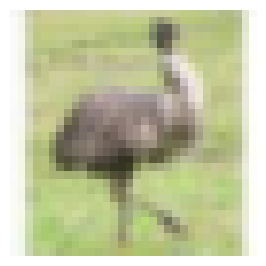
\includegraphics[width=\linewidth]{figures/cifar-images/bird.png}
      \centering\scriptsize\texttt{bird}
    \end{minipage} &
    \begin{minipage}[b]{0.15\linewidth}
      
\includegraphics[width=\linewidth]{figures/cifar-images/cat.png}
      \centering\scriptsize\texttt{cat}
    \end{minipage} &
    \begin{minipage}[b]{0.15\linewidth}
      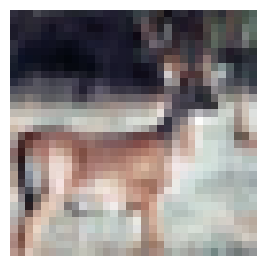
\includegraphics[width=\linewidth]{figures/cifar-images/deer.png}
      \centering\scriptsize\texttt{deer}
    \end{minipage} \\
    \begin{minipage}[b]{0.15\linewidth}
      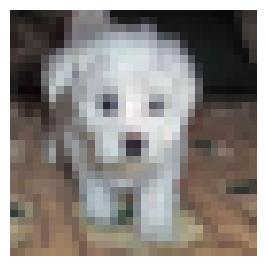
\includegraphics[width=\linewidth]{figures/cifar-images/dog.png}
      \centering\scriptsize\texttt{dog}
    \end{minipage} &
    \begin{minipage}[b]{0.15\linewidth}
      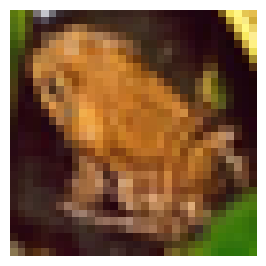
\includegraphics[width=\linewidth]{figures/cifar-images/frog.png}
      \centering\scriptsize\texttt{frog}
    \end{minipage} &
    \begin{minipage}[b]{0.15\linewidth}
      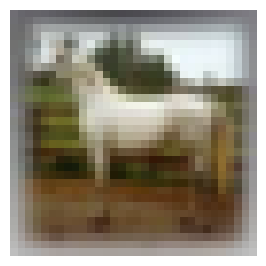
\includegraphics[width=\linewidth]{figures/cifar-images/horse.png}
      \centering\scriptsize\texttt{horse}
    \end{minipage} &
    \begin{minipage}[b]{0.15\linewidth}
      
\includegraphics[width=\linewidth]{figures/cifar-images/ship.png}
      \centering\scriptsize\texttt{ship}
    \end{minipage} &
    \begin{minipage}[b]{0.15\linewidth}
      
\includegraphics[width=\linewidth]{figures/cifar-images/truck.png}
      \centering\scriptsize\texttt{truck}
    \end{minipage}
  \end{tabular} 
\end{figure}
    \caption{Example images from CIFAR-10~\footfullciteieee{Krizhevsky2009}}
    \end{figure}
\end{columns}
}
\subsection{Datasets}
\begin{frame}{Datasets Used}
  \framesubtitle{CIFAR-10 Dataset}
  \vspace{-1em}
  \CifarDatasetSlide
\end{frame}
\note{

}

\newcommand{\DermPtDatasetSlide}[1]{
\begin{columns}[T]
  \column{\customcolumnwidth}
    \textbf{Dataset Characteristics}
    \vspace{-0.4em}
    \begin{itemize}
      \item 1,011 dermatological cases for melanoma diagnosis (as well as other skin conditions)
      \item Multiple image modalities:
        \begin{itemize}
          \item Dermoscopic (standardized)
          \item Clinical (varying conditions)
        \end{itemize}
      % \item Dataset split (diagnoses and features not uniform):
      %   \begin{itemize}
      %     \item 413 training cases
      %     \item 203 validation cases
      %     \item 395 test cases
      %   \end{itemize}
      \item Diagnoses and features are not uniformly distributed
      \item Task-specific dataset -- likely not present in VLM pre-training data
    \end{itemize}
  \column{\customcolumnwidth}
    \vspace{-0.5em}
    #1
\end{columns}
}

\newcommand{\DermPtFigureOne}{
  \begin{figure}[h]
    \centering
    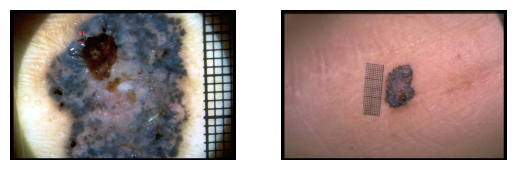
\includegraphics[width=0.9\linewidth]{figures/derm7pt-images/derm_01.png}
    \vspace{0.25em}
    \raggedright
    \scriptsize\texttt{diagnosis}: basal cell carcinoma\\
    \scriptsize\texttt{pigment\_network}: absent\\
    \scriptsize\texttt{streaks}: absent\\
    \scriptsize\texttt{pigmentation}: absent\\
    \scriptsize\texttt{regression\_structures}: blue areas\\
    \scriptsize\texttt{dots\_and\_globules}: irregular\\
    \scriptsize\texttt{blue\_whitish\_veil}: present\\
    \scriptsize\texttt{vascular\_structures}: within regression\\
    \vspace{0.25em}
    \scriptsize\texttt{seven\_point\_score}: 4\\
    \scriptsize\texttt{level\_of\_diagnostic\_difficulty}: low
    \caption{\centering An example case from Derm7Pt}
  \end{figure}
}

\newcommand{\DermPtFigureTwo}{
  \begin{figure}[h]
    \centering
    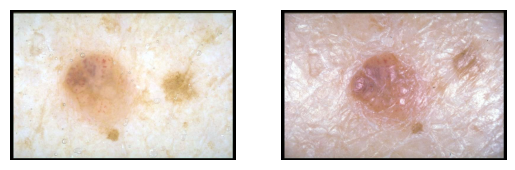
\includegraphics[width=0.9\linewidth]{figures/derm7pt-images/derm_02.png}
    \vspace{0.25em}
    \raggedright
    \scriptsize\texttt{diagnosis}: melanoma metastasis\\
    \scriptsize\texttt{pigment\_network}: absent\\
    \scriptsize\texttt{streaks}: absent\\
    \scriptsize\texttt{pigmentation}: diffuse irregular\\
    \scriptsize\texttt{regression\_structures}: absent\\
    \scriptsize\texttt{dots\_and\_globules}: regular\\
    \scriptsize\texttt{blue\_whitish\_veil}: absent\\
    \scriptsize\texttt{vascular\_structures}: hairpin\\
    \vspace{0.25em}
    \scriptsize\texttt{seven\_point\_score}: 1\\
    \scriptsize\texttt{level\_of\_diagnostic\_difficulty}: high
    \caption{\centering A particularly challenging example case from Derm7Pt}
  \end{figure}
}

\begin{frame}{Datasets Used}
  \framesubtitle{Seven-Point Checklist Dermatology Dataset (Derm7Pt)}
  \vspace{-1em}
  \DermPtDatasetSlide{\DermPtFigureOne}
\end{frame}
\note{
- The Derm7Pt dataset is a collection of dermatological images and annotations for melanoma diagnosis, as well as other skin conditions such as seborrheic keratosis, basal cell carcinoma, types of nevi, and more \\
- A seven point score of greater than or equal to 3 is to be referred for specialist analysis for melanoma \\
% - The example case shown is a melanoma metastasis case, but note that the seven point score is 1. This is a specifically challenging case, just to demonstrate the kind of examples that are present in the dataset \\
- The authors provide a python library as an interface to the dataset, and perform grouping of rare cases as well as the grouping of fine-grained categorization into more coarse categories \\
- In the authors' paper, it is shown that incorporating clinical images as input to their CNN model improves performance \\
}


\subsection{Models, Prompting Strategies}
\begin{frame}{Models and Prompting Strategies}
  % Content will be added later
\end{frame}